
%%%%%%%%%%%%%%%%%%%%%%% file typeinst.tex %%%%%%%%%%%%%%%%%%%%%%%%%
%
% This is the LaTeX source for the instructions to authors using
% the LaTeX document class 'llncs.cls' for contributions to
% the Lecture Notes in Computer Sciences series.
% http://www.springer.com/lncs       Springer Heidelberg 2006/05/04
%
% It may be used as a template for your own input - copy it
% to a new file with a new name and use it as the basis
% for your article.
%
% NB: the document class 'llncs' has its own and detailed documentation, see
% ftp://ftp.springer.de/data/pubftp/pub/tex/latex/llncs/latex2e/llncsdoc.pdf
%
%%%%%%%%%%%%%%%%%%%%%%%%%%%%%%%%%%%%%%%%%%%%%%%%%%%%%%%%%%%%%%%%%%%
%
%
%\documentclass[runningheads,a4paper]{llncs}
%
%\usepackage{amssymb}
%\usepackage{algorithm}
%\usepackage{algorithmic}
%\usepackage{dsfont}
%\usepackage{amsmath}
%\setcounter{tocdepth}{3}
%\usepackage{booktabs}
%\usepackage{multirow}
%\usepackage{graphicx}
%\usepackage{color}
%\usepackage[table]{xcolor}
%
%\usepackage{url}
%\urldef{\mailsa}\path|{agutierrez,eligius,igarciaf}@uma.es|
%\urldef{\mailsb}\path|gloriaortega@ual.es|
%\urldef{\mailsc}\path| {karin.pauls,rene.haijema}@wur.nl|
%\newcommand{\keywords}[1]{\par\addvspace\baselineskip
%\noindent\keywordname\enspace\ignorespaces#1}

\chapter{On computing order quantities for perishable inventory control with non-stationary demand} % top level followed by section, subsection
\label{Chap:iccsa2015}

\ifpdf
    \graphicspath{{X/figures/PNG/}{X/figures/PDF/}{X/figures/}}
\else
    \graphicspath{{X/figures/EPS/}{X/figures/}}
\fi

% NB: Chinese authors should write their first names(s) in front of
% their surnames. This ensures that the names appear correctly in
% the running heads and the author index.
%
%\author{Alejandro G. Alcoba \inst{1}
%\and Eligius M.T. Hendrix \inst{1}
%\and Inmaculada Garc\'ia\inst{1}
%\and Gloria Ortega \inst{2}
%\and Karin G.J. Pauls-Worm \inst{3}
%\and Rene Haijema \inst{3}}
%%
%\authorrunning{Alejandro G. Alcoba et al.}
%
%
%\institute{
%            Computer Architecture Dpt., Univ. of M{\'a}laga, 29080 M{\'a}laga, Spain\\
%             \mailsa
%            \and Informatics Dpt., Univ. of Almer\'ia, Agrifood Campus of Int. Excell., ceiA3, 04120 Almer\'ia, Spain \\
%            \mailsb
%           \and TI Food and Nutrition and Operations Research and Logistics, Wageningen University, The Netherlands\\
%            \mailsc
%}
%


%
%
%\toctitle{Lecture Notes in Computer Science}
%\tocauthor{Authors' Instructions}
%\maketitle

%---------------------------------------------------------------------------
%\begin{abstract}
%The determination of order quantities in an inventory control problem of perishable products with non-stationary demand can be formulated as a Mixed Integer Nonlinear Programming problem (MINLP). One of the challenges is to deal with the service level constraint in terms of the loss function. This paper studies the properties of the optimal solution and derives specific algorithms to determine (near) optimal quantities.
%
%
%\keywords{Inventory control, Perishable products, MINLP,  loss function, Monte Carlo}
%% \PACS{PACS code1 \and PACS code2 \and more}
%% \subclass{MSC code1 \and MSC code2 \and more}
%\end{abstract}

%-------------------------------------------------------------------------------
\section{Introduction}\label{sec:intro}
The basis of our study is a fill rate variant of a Stochastic Programming (SP) model presented in \cite{PAULS14} for a practical production planning problem over a finite horizon of $T$ periods of a perishable product with a fixed shelf life of $J$ periods. Items of age $J$ cannot be used at the next period and are considered waste. Demand is stochastic and non-stationary, as it changes over time. It is known (see \cite{kurawarwala96}), that inventory management under these circumstances raise the complexity of the model and make necessary the use of particular methods adapted to it.
To keep waste due to out-dating low, one issues the oldest product first, i.e. FIFO issuance. Literature provides many ways to deal with perishable products, order policies and backlogging, e.g. \cite{hedjar2004,Silver98}. The model we investigate aims to guarantee a service level constraint; the supplier guarantees to supply at least a fixed percentage of  the expected demand for every period. The demand that cannot be fulfilled is not backlogged.

The solution for such a model is a so-called order policy.
We consider a policy with a list of order periods $Y$ with order quantities  $Q_t$. The question is to derive a set of order quantities that leads to minimum cost and fulfills the service level constraint.

Section \ref{sec:model} introduces the model under study. Properties of the order quantities are studied in Section \ref{sec:rcot} where also a specific algorithm is derived to determine the so-called basic order quantities. Section \ref{sec:alg} then describes several algorithms to determine solutions, including an optimal one. Section \ref{sec:parameters} analyses the effect of the value of the parameters of the objective function on the optimal delivery orders. Finally, Section \ref{sec:conclusions} concludes and summarizes the findings.



\section{Stochastic Programming Model}
\label{sec:model}

The model describes the inventory development over $T$ periods, where $t$ is the time index and $j$ is the age of the product in inventory. The stochastic demand implies that the model has random inventory variables $\boldsymbol{I}_{jt}$ apart from the initial fixed levels $I_{j0}$. The model has to keep track of the lost sales $\boldsymbol{X}_t$ in periods where demand exceeds the available amount of product. Moreover, typical is the amount of product that perishes and becomes waste, $\boldsymbol{I}_{Jt}$. In the notation, %$P(.)$ denotes a probability to express the chance constraints and
$E(.)$ is the expected value operator. Moreover,  we use $x^+=max\{x,0\}$. A formal description of the SP model from \cite{PAULS14} is given.\\

\smallskip\noindent\emph{Indices}\\
\begin{tabular}{ll}
$t$ & period index, $t=1,\ldots,T$, with $T$ the time horizon\\
$j$ & age index, $j=1,\ldots,J$, with $J$ the fixed shelf life\\
\end{tabular}


\smallskip\noindent\emph{Data}\\
\begin{tabular}{ll}
$\boldsymbol{d}_t$ &
Normally distributed demand with mean value $\mu_t>0$ and variance  $(cv\times \mu_t)^2$\\
& where $cv$ is a given coefficient of variation.\\
$k$ & fixed ordering cost, $k>0$\\
$c$ & unit procurement cost, $c>0$\\
$h$ & unit inventory cost, $h>0$\\
$w$ & unit disposal cost, is negative when having a salvage value, $w>-c$\\
$\beta$ & service level, $0<\beta<1$
\end{tabular}

%\noindent 5pt

\smallskip\noindent\emph{Variables}\\
\begin{tabular}{ll}
$Q_t \ge 0$ & ordered and delivered quantity at the beginning of period $t$\\
$Y_t \in \{0,1\}$ & setup of order\\
$\boldsymbol{X}_t$ & lost sales in period $t$\\
$\boldsymbol{I}_{jt}$ & Inventory of age $j$ at end of period $t$, initial inventory fixed  $I_{j0}=0$,\\
 & $\boldsymbol{I}_{jt} \ge 0$ for $j=1,\ldots,J$.\\
\end{tabular}

\smallskip\noindent
The total expected costs over the finite horizon is to be minimized.

\begin{equation}
\label{eq:obj}
f(Q)=\sum_{t=1}^T \left(C(Q_t) + E\left(h\sum_{j=1}^{J-1} \boldsymbol{I}_{jt}  +w\boldsymbol{I}_{Jt}\right)\right),
%\sum_{t=1}^T g(Q_t) + E\left(h\sum_{t=1}^T \sum_{j=1}^{J-1} \boldsymbol{I}_{jt}^+ +w\boldsymbol{I}_{Jt}\right)=\sum_{t=1}^T g(Q_t) + E\left(h\sum_{j=1}^{J-1} \boldsymbol{I}^+_{jt}  +w\boldsymbol{I}_{Jt}\right),
\end{equation}
where procurement cost is given by the function
\begin{equation}
\label{eq:proc}
C(x) = k+cx, \ \ \text{if} \ \ x>0,\ \text{and}\ \ C(0)=0 .
\end{equation}
%
The FIFO dynamics of inventory of items of  age $j$ starts by defining waste ($j=J$)
\begin{equation}
\label{eq:invWaste}
\boldsymbol{I}_{Jt}=(\boldsymbol{I}_{J-1,t-1} - \boldsymbol{d}_t)^+, \ t=1,\ldots,T
\end{equation}
followed by the inventory of items with age $1<j<J$ that still can be used in the next period:
\begin{equation}
\label{eq:inv2}
\boldsymbol{I}_{jt}= \left(\boldsymbol{I}_{j-1,t-1} - (\boldsymbol{d}_t-\sum_{i=j}^{J-1}\boldsymbol{I}_{i,t-1})^+\right)^+, \ t=1,\ldots,T, j=2,\ldots,J-1 .
\end{equation}
%
and finally the incoming and freshest products, $j=1$:
%
\begin{equation}
\label{eq:inv1}
\boldsymbol{I}_{1t}= \left(Q_t - (\boldsymbol{d}_t-\sum_{j=1}^{J-1}\boldsymbol{I}_{j,t-1})^+\right)^+, \ t=1,\ldots,T.
\end{equation}
%
Lost sales for period $t$ is defined by
%
\begin{equation}
\label{eq:lostsales}
\boldsymbol{X}_t=\left(\boldsymbol{d}_t-\sum_{j=1}^{J-1}\boldsymbol{I}_{j,t-1}-Q_t\right)^+.
\end{equation}
%
The service level constraint for every period is
\begin{equation}
\label{eq:chance}
E \left(\boldsymbol{X}_t\right) \le (1-\beta) \mu_t, \ t=1,\ldots,T.
\end{equation}
%
Notice that given the stochastic variables of demand, the expectation of lost sales only depends on the ordered quantities $Q: (Q_1,\ldots, Q_T)$. For a MINLP approach, we can also express these constraints as follows
%
\begin{equation}
\label{eq:defg}
g_t(Q)=E \left(\boldsymbol{X}_t\right) - (1-\beta)\mu_t\le 0,\ t=1,\ldots,T.
\end{equation}
%
We consider a simple order policy, where the decision maker should provide an integer vector $Y=(Y_1,\ldots,Y_T)\subset \{0,1\}^T$ of order periods and order quantities $Q_t$ with $t=1,\ldots,T$ where $Y_t=0$ implies $Q_t=0$. This can be considered a MINLP problem to derive what are the optimal values of the (continuous) order quantities $Q_t$ and the corresponding optimal (integer) order timing $Y$. In summary, we have a $MINLP (Q)$ problem:
$\min_Q f(Q)$
subject to the inventory development (\ref{eq:invWaste}), (\ref{eq:inv2}), (\ref{eq:inv1}), (\ref{eq:lostsales}) and $g_t(Q)\le 0,\ t=1,\ldots,T$.




\section{Replenishment cycles and basic order quantities}
\label{sec:rcot}
%
We study several theoretical properties of the order quantities $Q$ and the list of order periods $Y$. We first focus on the concept of replenishment cycles in Section \ref{sec:repl} and determine in which cases a so-called basic order quantity defines the optimal order quantity in Section \ref{sec:safe}. Section \ref{sec:nlp} then derives properties of the optimal quantities given a timing vector $Y$, which can be used in the design of specific algorithms in Section \ref{sec:alg}.


\subsection{Feasible replenishment cycles}
\label{sec:repl}

Literature on inventory control (e.g. \cite{Silver98}) applies the concept of a replenishment cycle, i.e. the length of the period $R$ for which the order of size $Q$ is meant. For stationary demand, the replenishment cycle is fixed, but for non-stationary demand the optimal replenishment cycle may depend on the period.
 \begin{defn}
 \label{def:A}
Given a list of order periods $Y\in \{0,1\}^T$ and $N=\sum_{t=1}^T Y_t$. The order timing vector $A \in \mathbb{N}^N$ for $Y$ gives the periods $A_i< A_{i+1}$ where  $Y_{A_i}=1$.
\end{defn}
%
\begin{defn}
 \label{def:R}
Given a list of order periods $Y\in \{0,1\}^T$ with total number of orders $N=\sum_{t=1}^T Y_t$. Replenishment cycle $R_i=A_{i+1}-A_i, \ i=1,\ldots,N-1$ and $R_N=T-A_N+1$.
\end{defn}
Notice that for the perishable case with a shelf life $J$, to fulfill the service level constraint, practically the replenishment cycle cannot be larger than the shelf life $J$; so $1 \le R_i \le J$.
\begin{lemma}
\label{lem:Y}
Let $Y$ be an order timing vector of the SP model, i.e. $Y_t=0 \Rightarrow Q_t=0$. $Y$ provides an infeasible solution of the SP model, if it contains more than $J-1$ consecutive zeros.
\end{lemma}
This means that a feasible order timing vector $Y$ does not contain a consecutive series with more than $J-1$ zeros.

\begin{defn}
We define $F_T$ as the set of all feasible order timing vectors $Y$ of length $T$.
\end{defn}

For the given model the number of elements $|F_T|$, for $T\leq J$ is equal to $2^{T-1}$. Given the assumption of zero starting inventory, an element $Y\in F_T$ must start with $Y(1)=1$, otherwise demand will not be satisfied for the first period. From here, any combination is valid, since there are no more than $J-1$ elements to consider. The case $T=J+1$ is slightly different: for the first period again $Y(1)=1$ is needed, and for the rest of elements there are $2^J$ possible cases, and only the one with $J$ zeros is not feasible, so $|F_{J+1}|=2^J-1$.

For $T>J+1$ the number of feasible series can be derived recursively according to the following proposition.
\begin{proposition}
\label{prop:numberfeasible}
The number of elements $|F_T|$ of the set $F_T$ of feasible order timings of $T$ periods and a shelf life $J$ with $J+1<T$ follows the recursive rule

\begin{equation}
\label{eq:numberfeasibleY(T)}
|F_{T+1}|= 2|F_{T}| -|F_{T-J}|
\end{equation}
with the initial terms  $|F_{t}|=2^{t-1} \  t<J+1$and  $|F_{J+1}|=2^J-1 $
\end{proposition}

\begin{proof}

Consider $p=(p_1,\ldots,p_{T})\in F_{T}$, then obviously $(p_1,\ldots,p_{T},1)\in F_{T+1}$. We now focus on the case of $(p,0)=(p_1,\ldots,p_{T},0)$. Its feasibility is determined by the values of $p_{T-(J-2)},\ldots, p_{T-1},p_T$. Let $\boldsymbol{0}$ be now an all zeros vector with $J-1$ elements. If $(p_{T-(J-2)},\ldots, p_{T-1},p_T)=\boldsymbol{0}$, then $(p,0)$ is not feasible. But how many feasible $p\in F_{T}$ exist with this feature?

Given $(p_{T-(J-2)},\ldots, p_{T-1},p_T)=\boldsymbol{0}$ and $p\in F_{T}$, we must have $p_{T-J+1}=1$. There are $|F_{T-J}|$ feasible timing vectors $(p_1,\ldots,p_{T-J})$, such that $(p_1,\ldots,p_{T-J},1,\boldsymbol{0})$ is feasible and  $(p_1,\ldots,p_{T-J},1,\boldsymbol{0},0)$ is infeasible.
Doing the bookkeeping correctly, this provides us with $|F_{T+1}|= 2|F_{T}| -|F_{T-J}|$.
$\blacksquare$
\end{proof}




The proof of Proposition~\ref{prop:numberfeasible} gives a constructive method to determine all feasible policies recursively. Moreover, (\ref{eq:numberfeasibleY(T)}) shows that the space of feasible policies grows exponentially with $T$ as illustrated in Figure~\ref{fig:numberfeasible}.

\begin{figure}[!bt]
\centering
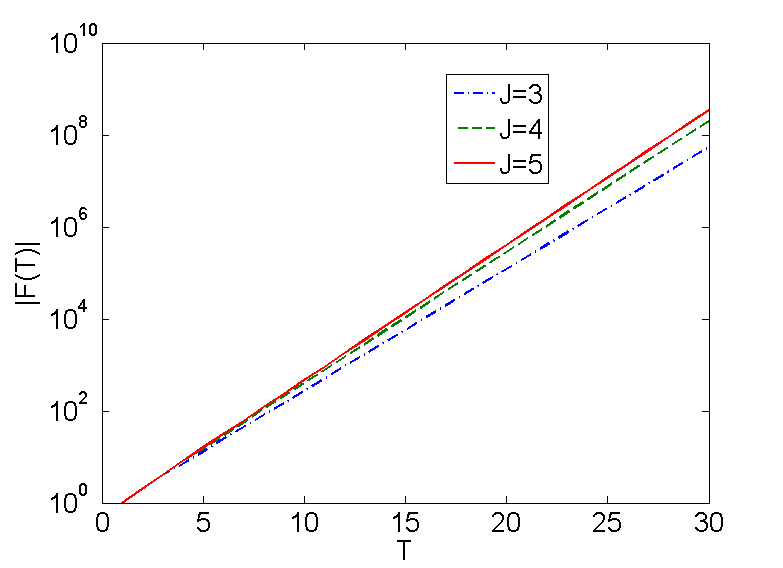
\includegraphics[scale=0.3]{iccsa2015/figures/numberfeasiblelogy.png} % escala semilogaritmica
%\includegraphics[scale=0.5]{numberfeasible.png} %escala normal (equi)
\caption{ $|F(T)|$ as a function of $T$ and several values of the shelf life $J$.}
\label{fig:numberfeasible}
\end{figure}


\subsection{Basic order quantities}
\label{sec:safe}
We focus now on the minimum order quantity at any period $t\in \{1,\ldots,T\}$ that is just sufficient to cover the demand according to the service level constraint for the next $r$ periods $t, t+1,\ldots, t+r-1$ considering that at period $t$ no older product is in stock.
\begin{defn}
Basic order quantity $\overline Q_{r,t}$ is the amount for period $t$ that fulfills constraint (\ref{eq:chance}) for the next $r$ periods: $t,t+1,\ldots,t+r-1$.
\end{defn}
We first consider $\overline Q_{1t}$. Let the replenishment cycle be one period $R=1$, zero inventory and $q$ the order quantity. In this case, lost sales $X$ from expression (\ref{eq:lostsales}) can be simplified to:
%
\begin{equation}
\boldsymbol{X}=\left(\boldsymbol{d}-q\right)^+ .
\end{equation}
Let $\varphi$ be the density function (pdf) of $\boldsymbol d$ and $\Phi$ be the corresponding cumulative distribution function (cdf).
%
Then the so-called loss function expressing the expected lost sales as a function of $q$ is
%
\begin{equation}
L(q) = E(\boldsymbol{X})=E\left((\boldsymbol{d}-q)^+\right)= \int\limits_{q}^{\infty} (x-q)\varphi(x)dx,
\end{equation}
%
where the symbol $x$ is used here as the argument in the integral. The cost function (\ref{eq:obj}) is monotonously increasing in the order quantity $q$ and $L(q)$ decreases, so constraint (\ref{eq:chance}) is binding for the optimal value of $q$ such that $L(q) = (1-\beta) \mu$ as illustrated in Figure~\ref{fig:lossfunFig}. Since demand is normally distributed, there is no closed-form expression for the first order loss function and the solution has to be calculated numerically. Some approximations for the loss function can be found in  \cite{kurawarwala96},\cite{Rossi14},\cite{DeSchrijver20121375},\cite{Waissi199691}. From a root-finding perspective, there are several ways to proceed (see \cite{HENTO10}). For instance, one can use the derivative of loss function  $L'(q)=\int\limits_{-\infty}^{q}\varphi(x)dx - 1 = \Phi(q) - 1$ to approximate $q$ using \emph{Newton Raphson}. The following theoretical result shows that for the described model, the determination of $q$ has to be done only once.
%
\begin{figure}[!bt]
\centering
%\includegraphics[scale=0.5]{lossfunction.png}
\includegraphics[scale=0.3]{iccsa2015/figures/lossfunFig.png}
%\includegraphics[scale=0.5]{lossfunFig.pdf}
\caption{One period loss function $E(X|Q)$ for $\boldsymbol d \sim N(1950,0.25\cdot1950)$ and corresponding basic order quantity $q$: $E(X|q)=(1-\beta)\mu$}
\label{fig:lossfunFig}
\end{figure}
%
\begin{lemma}
\label{lem:q1}
Let $\boldsymbol{d}\sim N(\mu,cv\times \mu)$ and $\varphi$ be the pdf and $\Phi$ the cdf of the standard normal distribution. The solution of  $L(q) = (1-\beta) \mu$ fulfills $q=\mu(1+cv\times\hat x)$ where $\hat x$ solves
$\varphi\left(\hat x\right)-\left(1-\Phi\left(\hat x\right)\right)\hat x =\frac{1-\beta}{cv}$.
\end{lemma}
%
\begin{proof}
Using the results in \cite{Rossi14} for $\boldsymbol{d}\sim N(\mu,cv\times\mu)$,  the loss function can be expressed as
%
\begin{equation}
\label{eq:rossi}
L(q)=cv\times\mu \left(\varphi\left(\frac{q-\mu}{cv\cdot\mu}\right)-\left(1-\Phi\left(\frac{q-\mu}{cv\cdot\mu}\right)\right)\frac{q-\mu}{cv\cdot\mu}\right) .
 \end{equation}
The Equation $L(q)=(1-\beta)\mu$ substituting $q=\mu(1+cv\times\hat x)$ implies
%
\begin{equation}
\label{eq:rossi2}
 \varphi\left(\frac{q-\mu}{cv\cdot \mu}\right)-\left(1-\Phi\left(\frac{q-\mu}{cv\cdot \mu}\right)\right)\frac{q-\mu}{cv\cdot \mu} =
\varphi(\hat x)-(1-\Phi(\hat x))\hat x =
 \frac{1-\beta}{cv} .
 \end{equation}
$\blacksquare$
\end{proof}
%
\begin{figure}[!bt]
\centering
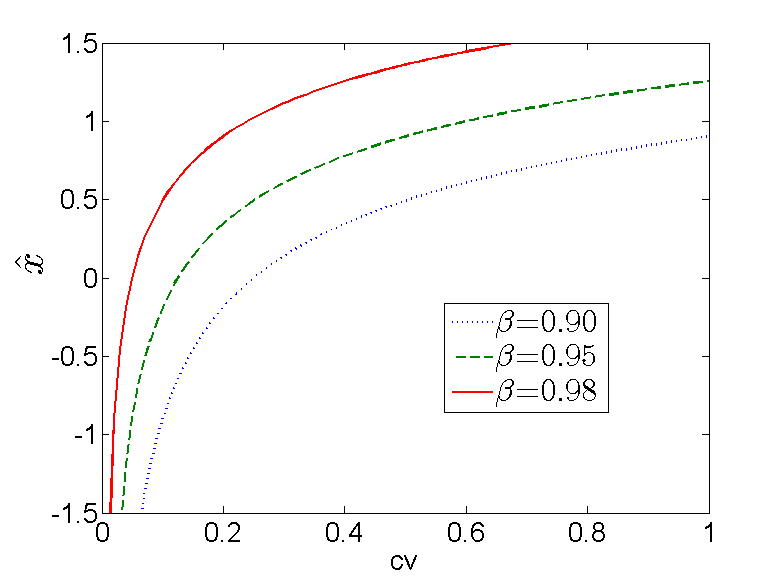
\includegraphics[scale=0.30]{iccsa2015/figures/xhat_ncvnew.png}
%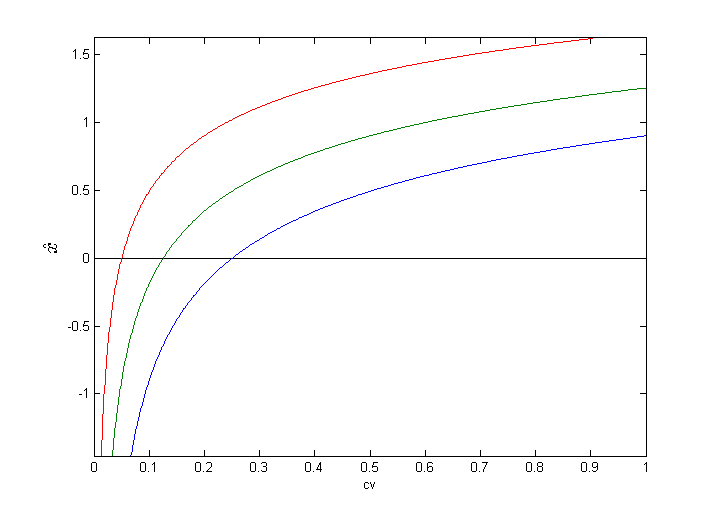
\includegraphics[scale=0.4]{xhat_ncv.pdf}
\caption{Values of $\hat x$, from solving Equation \ref{eq:rossi2} are represented  as a function of $cv$ for several values of $\beta=0.90, \ 0.95, \ 0.98$ %(blue) $\beta=0.95$ (green) and $\beta=0.98$ (red)
}
\label{fig:xhat_ncv}
\end{figure}
%
The basic order quantity $\overline Q_{1t}= \mu_t(1+cv\times\hat x)$ provides an upper bound on the order quantity $Q_t$ if $R_t=1$, because inventory may be available. Figure~\ref{fig:xhat_ncv} shows the relation of $\hat x$ with parameters $cv$ and $\beta$. Values greater than 0 mean that the basic quantity is greater than $\mu$.

The basic order quantities for longer replenishment cycles look more complicated. For instance, $R_t=2$ implies
$$E\left(\boldsymbol{d}_{t+1}-(\overline Q_{2t}-\boldsymbol{d}_{t})^+)\right)^+=(1-\beta)\mu_{t+1}$$
%
These expressions grow in complexity with the size of the replenishment period. To solve them we need a different approach.
%
Consider a replenishment cycle of $r$ periods, from $t_1$ to $t_2$ with $t_2=t_1+r-1$ and $\boldsymbol{d_{t_1,t_2}} = \boldsymbol {d_{t_1}} + \ldots + \boldsymbol {d_{t_2}}$.  Let $\varphi_{t_1,t_2}$ be the density function (pdf) of $\boldsymbol d_{t_1,t_2}$ and $\Phi_{t_1,t_2}$ be the corresponding cumulative distribution function (cdf). As we are considering that demand is normally distributed, the distribution of $\boldsymbol d_{t_1,t_2}$ is normal as well, with expected value $\mu=\mu_{t_1} + \ldots + \mu_{t_2}$ and $\sigma=cv \sqrt{\mu^2_{t_1} + \ldots+\mu^2_{t_2}}$. Starting with $q$ units at period $t_1$, the expected value of the sum of lost sales from periods $t_1$ to $t_2$, $SL_{t_1,t_2}(q)$ is determined by
\begin{equation}
\label{eq:sumloss}
SL_{t_1,t_2}(q)=E\left(\sum\limits_{i=t_1}^{i=t_2}X_i\right) =E\left((\boldsymbol{d_{t_1,t_2}}-q)^+\right)= \int\limits_{q}^{\infty} (x-q)\varphi_{t_1,t_2}(x)dx.
\end{equation}
Following the considerations in \cite{Rossi14}, $SL_{t_1,t_2}(q)$ can be expressed as
%
\begin{equation}
\label{eq:rossitotloss}
SL_{t_1,t_2}(q)=\mu-q+\sigma\varphi\left(\frac{q-\mu}{\sigma}\right)+\Phi\left(\frac{q-\mu}{\sigma}\right)(q-\mu),
 \end{equation}
% where $\mu=\mu_{t_1} + \ldots + \mu_{t_2}$ and $\sigma=cv \sqrt{\mu^2_{t_1} + \ldots+\mu^2_{t_2}}$.
Now consider the expected lost sales $L_{t_1,t_2}(q)$ in period $t_2$ when $q$ fresh units are available at the beginning of period $t_1$. The quantity follows from subtracting from the expected total lost sales up to period $t_2$ in (\ref{eq:sumloss}) the expected value of total lost sales from periods $t_1$ to $t_2 -1$
\begin{eqnarray}
\label{eq:lostsalesgeneral}
L_{t_1,t_2}(q)&=& SL_{t_1,t_2}(q)- SL_{t_1,t_2-1}(q) = \\ \nonumber
&&=\int\limits_{q}^{\infty} (x-q)\left(\varphi_{t_1,t_2}(x)-\varphi_{t_1,t_2-1}(x)\right)dx.
\end{eqnarray}
To find the value $q_{rt}$ for which the service level constraint is just fulfilled in period $t_2=t+r-1$ when having $q_{rt}$ fresh units at the beginning of period $t$ follows from solving $L(q_{1t})=(1-\beta)\mu_t$ according to Lemma \ref{lem:q1} and for $r>1$ one can solve
\begin{equation}
\label{eq:partialbasic}
SL_{t,t+r-1}(q_{rt})-SL_{t,t+r-2}(q_{rt})=(1-\beta)\mu_{t+r-1}
 \end{equation}
 for $q_{rt}$. The basic order quantity $\overline Q_{rt}$ now follows from taking the maximum of these quantities $\overline Q_{rt}=\max_{j=1,\ldots,r}q_{jt}$, such that the service level constraint is fulfilled in all periods of the replenishment cycle. Example \ref{ex:mainexample} sets values for the parameters and variables needed to be able to build a table with all the basic order quantities.
%%%%%%



\begin{example}
\label{ex:mainexample}

%\begin{table}
%\caption{Basic order quantities}
%\begin{tabular}{ c | c  p{0.4cm} p{0.4cm} p{0.4cm} p{0.4cm} p{0.4cm} p{0.4cm} p{0.4cm} p{0.4cm} p{0.4cm} p{0.4cm}  p{0.4cm}}
%\label{tab:demand}
%%\tiny
%\small
%\backslashbox{r}{t}  & 1 & 2 & 3 & 4 & 5 & 6 & 7 & 8 & 9 & 10 & 11 & 12\\
%%R & 1 & 2 & 3 & 4 & 5 & 6 & 7 & 8 & 9 & 10 & 11 & 12\\
%\hline
%1 & 899 & 1068 & 225 & 1011 & 899 & 169 &	731 & 899 & 1011 & 337 & 169 & 674\\
%2 & 1954 & 1464 & 1218 & 1925 & 1219 & 885 & 1618 & 1904 & 1467 & 532 & 830 & 0\\
%3 & 2380 & 2293 & 2130 & 2283 & 1803 & 1772 & 2608 & 2384 & 1680 & 1150 & 0 & 0 \\
%\hline
%$\mu_t$ & 800 & 950 & 200 & 900 & 800 & 150 & 650 & 800 & 900 & 300 & 150 & 600 \\
%\hline
%\end{tabular}
%\end{table}


As an example we will consider an instance of the problem of $T=12$ periods and shelf life $J=3$.
Random variables of demand for every period are expressed in terms of their mean values $\mu_t$ that are given in last row of Table \ref{tab:demand} and the coefficient of variation is given by $cv=0.25$. Consider a service level of $\beta=95\%$, then the value of $\hat x$ in Lemma \ref{lem:q1} is $\hat x=0.493$. This value can be used to determine the values for $\overline Q_{1t}$, the first row in Table \ref{tab:demand}. Solving (\ref{eq:partialbasic}) and taking  $\overline Q_{rt}=\max_{j=1,\ldots,r}q_{jt}$ provides values for $\overline Q_{rt}$ for $r>1$ in Table \ref{tab:demand}. The values are rounded up.
%
\end{example}

\begin{table}[bt!]
	\caption{Basic order quantities $\overline Q_{rt}$ and mean period demands $\mu_t$}
	\label{tab:demand}
    \centering
	\begin{tabular}{@{}lrrrrrrrrrrrr@{}}
		\toprule
		t        & \multicolumn{1}{c}{1} & \multicolumn{1}{c}{2} & \multicolumn{1}{c}{3} & \multicolumn{1}{c}{4} & \multicolumn{1}{c}{5} & \multicolumn{1}{c}{6} & \multicolumn{1}{c}{7} & \multicolumn{1}{c}{8} & \multicolumn{1}{c}{9} & \multicolumn{1}{c}{10} & \multicolumn{1}{c}{11} & \multicolumn{1}{c}{12} \\ \midrule
		$\overline Q_{1t}$ & 898                   & 1067                  & 224                   & 1010                  & 898                   & 168                   & 730                   & 898                   & 1010                  & 336                    & 168                    & 673                    \\
		$\overline Q_{2t}$ & 1952                  & 1450                  & 1211                  & 1925                  & 1225                  & 885                   & 1618                  & 1898                  & 1458                  & 529                    & 825                    & 0                      \\
		$\overline Q_{3t}$ & 2372                  & 2277                  & 2131                  & 2287                  & 1812                  & 1769                  & 2596                  & 2386                  & 1666                  & 1145                   & 0                      & 0                      \\ \midrule
		$\mu_t$  & 800                   & 950                   & 200                   & 900                   & 800                   & 150                   & 650                   & 800                   & 900                   & 300                    & 150                    & 600
	\end{tabular}
\end{table}



\subsection{Optimal quantities for a given $Y$}
\label{sec:nlp}
So far, we have described %an Algorithm (\ref{alg:feasible}) that gives
a method to find a feasible $Q$ vector for a given $Y$, using the so called Basic order quantities. Now we can define a method to optimize the objective function (\ref{eq:obj}) subject to a given timing vector $Y$.

We consider now the properties of the MINLP problem described in Section \ref{sec:model}. We first focus on the monotonicity of the objective function in the order quantities when $w>-c$ applies.



%\begin{lemma}
%\label{lem:ineq_g}
%\green{Consider a replenishment cycle for periods $t_1$ to $t_2=t_1+R-1$ and $Q\in  \mathbb{R}^+$. Then,}
%
%\begin{equation}
%g_{t_1}(Q)\leq g_{t_1+1}(Q)\leq \ldots \leq g_{t_2}(Q)
%\end{equation}
%\end{lemma}
%\begin{proof}
%\green{content...}
%\end{proof}



\begin{proposition}
\label{prop:optimizeY}
Let $Q^*(Y)$ be an optimal solution of (\ref{eq:obj}),(\ref{eq:proc}),(\ref{eq:invWaste}), (\ref{eq:inv2}), (\ref{eq:inv1}), (\ref{eq:lostsales}) and (\ref{eq:defg}) with the restriction that $Q_t= 0$ if $Y_t=0$.  The optimum value $Q^* =(Q_1^*,\ldots, Q_{T}^*)= min_Q f(Q_1 ,\ldots, Q_{T})$ is reached iff:
\begin{equation}
\label{eq:optimalQ}
%Q^* =(Q_1^*,\ldots, Q_{T}^*)= min_Q f(Q_1 ,\ldots, Q_{T})\\
 %\text{ s.t. }
 g_{A_2-1}(Q^*) = \ldots = g_{A_N-1}(Q^*)= g_{A_T}(Q^*)=0 %\nonumber
\end{equation}
where $A \in \mathbb{N}^N$ is the vector of order periods for $Y$.
\end{proposition}




\begin{proof}
To prove that $Q^*$ is the optimal solution for any value of the parameters ($k,c,h,w$) of the objective function $f(Q)$ (see (\ref{eq:obj})), we will show that $Q^*$ is optimal for the ordering cost $f_k(Q)= k\sum_{t=1}^T Y_t $  ($f$ setting  $c=h=w=0$), also for the procurement cost plus the waste cost $f_{c,w}(Q)=\sum_{t=1}^T \left(c Q_t+ E\left(w\boldsymbol{I}_{Jt}\right)\right)$ ($f$ setting $k=h=0$) and for the inventory cost $f_h(Q)=\sum_{t=1}^T E\left(h\sum_{j=1}^{J-1} \boldsymbol{I}_{jt} \right)$ ($f$ setting $k=c=w=0$).







The ordering cost for $Q^*$ is $f_k(Q^*)=k\sum\limits_{t=1}^{T}Y_t$ only depends on the timing vector $Y$ and hence $Q^*$ has the same ordering cost than any other feasible solution subject to  $Y$.

The expected value of perished items, $E\left(\boldsymbol{I}_{Jt}\right)$, with $t=1,\ldots,T$ are just a part of the total quantity produced $S(Q)=\sum\limits_{t=1}^{T}Q_t$ and this, joined with the restriction $w>-c$ implies that the procurement and disposal cost, $f_{c,w}(Q)=\sum_{t=1}^T \left(c Q_t+ E\left(w\boldsymbol{I}_{Jt}\right)\right)$, decreases with $S(Q)$. At the same time, the hold inventory depends on  $Q$, and it is minimum when the amount $S(Q)$ is minimum as well.

We will show now that $Q^*$ minimizes the total quantity produced for all the periods.
In Section \ref{sec:safe} we described analytically the loss function for different replenishment cycles lengths and we showed that it decreases as a function of the quantity added. Then, for any order period $Q_{A_i}$, $i=1,\ldots,N$, the value of  $E(X)$ decreases with $Q_{A_i}$ for all the periods of the replenishment and hence constraint function $g$ decreases with $Q_{A_i}$ for these periods as well. For $Q^*$ as described in (\ref{eq:optimalQ}) the total amount $S(Q^*)$ reaches its minimum value. $\blacksquare$

%For $Q^*$ as described in (\ref{eq:optimalQ}) none of the values $Q_{A_i}$ can be taken lower than $Q_{A_i}^*$ \red{independently (it would cause infeasibility since, by Lemma \ref{lem:ineq_g}, $Q^*_{A_i}$ is the minimal value that fulfill the $\beta$ service level for all the periods of the cycle). It is possible, though, to raise the production value of one (or several) order periods in order to have the chance, by having a greater inventory, to reduce the quantity in a later order period  $Q_{A_i}$ below the value of $Q_{A_i}^*$, but obviously never as much as the raise of previously produced. $\blacksquare$}

\end{proof}

Notice that (\ref{eq:optimalQ}) implicitly states how to calculate $Q^*$: Starting for the quantity of the first cycle, and taking it as low as constraint (\ref{eq:chance}) is fulfilled and so on until the last cycle. We must emphasise again that, given $Y$, the optimal quantities do not depend on the parameters of the objective function (\ref{eq:obj}).



\section{Algorithms for generating order quantities}
\label{sec:alg}

The derived basic order quantities can now be used to obtain feasible solutions and to improve them towards (near) optimal solutions.

\subsection{Generating a feasible solution for a given $Y$}
Given a list of order periods $Y$ we can determine a feasible solution $Q$ provided by the $\overline{Q}_{r,t}$ values, with $r\in\{1,\ldots,J\}$ and $t\in \{1,\ldots,T\}$.
 After we calculate vectors $A$ and $R$ from Definitions \ref{def:A} and \ref{def:R} we just need to assign the correct values.  Creating an algorithm to build feasible solutions is straightfoward. At Example \ref{ex:feasiblesolY} we show a single case for a vector $Y$.


\begin{example}
\label{ex:feasiblesolY}
Considering the same data and variables of Example \ref{ex:mainexample}, we can easily determine the order  quantities $Q_t$ for building a feasible solution for any timing vector $Y$ using the basic order quantities $\overline Q_{r,t}$. For instance, considering the timing vector $Y=(1,1,0,1,0,1,1,0,1,1,1,0)$, the resulting output is  $Q=(898,1450,0,$ $1925,0,168,$ $1618,0,1010,$ $336,825,0)$, where the appropiate basic order quantities have been chosen, as we can see at Table \ref{tab:Ybasicorder}.
\end{example}


\begin{table}[bt!]
	\caption{Election of basic order quantities for a particular $Y$}
	\label{tab:Ybasicorder}
	\begin{tabular}{@{}lrrrrrrrrrrrr@{}}
		\toprule
		t        & \multicolumn{1}{c}{1} & \multicolumn{1}{c}{2} & \multicolumn{1}{c}{3} & \multicolumn{1}{c}{4} & \multicolumn{1}{c}{5} & \multicolumn{1}{c}{6} & \multicolumn{1}{c}{7} & \multicolumn{1}{c}{8} & \multicolumn{1}{c}{9} & \multicolumn{1}{c}{10} & \multicolumn{1}{c}{11} & \multicolumn{1}{c}{12} \\ \midrule
		$\overline Q_{1t}$ & \textbf{898}          & 1067                  & 224                   & 1010                  & 898                   & \textbf{168}          & 730                   & 898                   & \textbf{1010}         & \textbf{336}           & 168                    & 673                    \\
		$\overline Q_{2t}$ & 1952                  & \textbf{1450}         & 1211                  & \textbf{1925}         & 1225                  & 885                   & \textbf{1618}         & 1898                  & 1458                  & 529                    & \textbf{825}           & 0                      \\
		$\overline Q_{3t}$ & 2372                  & 2277                  & 2131                  & 2287                  & 1812                  & 1769                  & 2596                  & 2386                  & 1666                  & 1145                   & 0                      & 0                      \\ \midrule
		$\mu_t$  & 800                   & 950                   & 200                   & 900                   & 800                   & 150                   & 650                   & 800                   & 900                   & 300                    & 150                    & 600
	\end{tabular}
\end{table}

\subsection{Generating the optimal solution for a given $Y$}

The process of optimizing quantities for a timing vector $Y$ is sketched at Algorithm \ref{alg:optimalforY}. Proposition \ref{prop:optimizeY} establishes implicitly at (\ref{eq:optimalQ}) that the quantities for the order periods of $Y$ must be calculated sequentially from the first one, $A_1=1$,  to the last, $A_M$, where $M$ is $\sum\limits_{j=1}^{T}Y_j$. If a replenishment period $A_i$ is preceded by exactly $J-1$ periods without replenishment, it is obvious that inventory at $A_i$ would be deterministic and equal to zero due to the expiration of stock. In those cases the basic order quantity $Q_{R_i,A_i}$ (being $R_i$ the length of the replenishment cycle $i$) is optimal, as constraint  (\ref{eq:chance}) would be adjusted to the minimum. Otherwise, when a period $A_i$ is preceded by less than $J-1$ periods since last replenishment, the optimal order quantity is lower that the one given by the basic order for that cycle, due to the previous inventory random variables $\boldsymbol{I}_{1,A_{i}-1}\ldots,\boldsymbol{I}_{J-1,A_{i}-1}$, that allow us to reduce the basic order value up to the minimum allowed by constraint (\ref{eq:chance}) for that  cycle. In these cases, lost sales cannot be obtained by Equation (\ref{eq:lostsalesgeneral}), as it only holds when there is no inventory, but we can estimate that value through simulations.

\begin{algorithm}[!bt]
	\caption{MinQ($Y$): Optimal order quantity $Q$ for $Y$}
	\label{alg:optimalforY}
	\begin{algorithmic}[1]
		%\Procedure{MinQ}{$Y$}
        \REQUIRE Orders timing ($Y$), number of periods ($T$), fixed shelf life ($J$) and number of orders of a particular $Y$($M$)
        \ENSURE Optimal order quantity $Q$ for $Y$
        \medskip
		\STATE Generate the replenishment periods ($A$) for the given $Y$
        \STATE Generate  the length of the replenishment cycle ($R$) for the given $Y$
		\FOR {$i=1$ \textbf{to} $M$ } % For every vector of order periods for $Y$
        \IF  { ($A_i=1$ \textbf{or} $A_i -  A_{i-1}=J$) }  %[Inventory is zero] %\hfill \#Inventory is zero
		\STATE $Q_i=Q_{R_i,A_i}$; \label{optimalforY:line:beforefloss} \hfill \#Constraint~(\ref{eq:chance}) is adjusted to the minimum
		\STATE  \textbf{floss}($Q_i,A_i,A_i+R_i-1$) \label{optimalforY:line:floss} \hfill \# Algorithm~\ref{alg:simulation}: Update the inventory ($I$)
		\ELSE
        \STATE $Q_i=$ \textbf{Ordervalue}($A_i,R_i$) \hfill \# Algorithm~\ref{alg:ordervalue}
		\ENDIF
		\ENDFOR
		%\EndProcedure
		\vskip 5pt
	\end{algorithmic}
	
\end{algorithm}




Algorithm~\ref{alg:simulation} is based on the method of Monte Carlo. Function floss($q$,$t_1$,$t_2$)  consists of simulating $N$ times the evaluation of the inventory and the lost sales from period $t_1$ to $t_2$, for an order quantity of $q$ at the beginning of period $t_1$. To do so it generates $N$ samples of demand for each period and Equations (\ref{eq:invWaste}), (\ref{eq:inv2}), (\ref{eq:inv1}) and (\ref{eq:lostsales}) are used to update inventory and lost sales variables for each simulation. Function \emph{floss} returns the  estimated value of the expected lost sales  at the last period $X_{t_2}$. %, the one that by lemma \ref{lem:ineq_g} we have to adjust to the minimum.
%for the periods considered.
 Notice that in Algorithm \ref{alg:optimalforY} (line~\ref{optimalforY:line:floss}), even when an order quantity is obtained by a basic order quantity (line~\ref{optimalforY:line:beforefloss}), the Algorithm~\ref{alg:simulation} must be run once  to update the inventory ($I$) at the end of the cycle (period $t_2$). The value of $N$ must be large enough to provide accurate values for the lost sales.




\begin{algorithm}[!hbt]
	\caption{floss($q$,$t_1$,$t_2$): Monte Carlo simulation to update $\boldsymbol{I}$ and $\boldsymbol{X}$}
	\label{alg:simulation}
	\begin{algorithmic}[1]
        \REQUIRE Order quantity ($q$), initial ($t_1$) and final ($t_2$) periods of the simulation, number of simulations ($N$), fixed shelf life ($J$) of the perishable products, inventory ($I$), optimal order quantity for $Y$ ($Q$), normally distributed demand ($d$) and lost sales ($X$)
        \ENSURE  Estimated expected lost sales at the last period ($E(X_{t_2})=\frac{1}{N}\sum\limits_{n=1}^{N}X_{t_2n}$)
        \medskip
		\FOR{$n=1$ \textbf{to} $N$}
			\FOR{$t=t_1$ \textbf{to} $t_2$}
				\FOR{$j=2$ \textbf{to} $j=J-1$ }
					\STATE $I_{j,t,n}= \left(I_{j-1,t-1,n} - (d_{t,n}-\sum_{k=j}^{J-1}I_{k,t-1,n})^+\right)^+$; \hfill \#Update inventory ($I$)
				\ENDFOR
				\STATE $I_{1,t,n}= \left(Q_t - (d_{t,n}-\sum_{j=1}^{J-1}I_{j,t-1,n})^+\right)^+$; \hfill \#Update inventory ($I$)
				\STATE $I_{J,t,n}=(I_{J-1,t-1,n} - d_{t,n})^+$
				\STATE $X_{t,n}=\left(d_{t,n}-\sum_{j=1}^{J-1}I_{j,t-1,n}-q\right)^+$; \hfill \#Update lost sales $X$
			\ENDFOR
		\ENDFOR
		\vskip 5pt
	\end{algorithmic}
	
\end{algorithm}


To calculate the order quantities for a timing vector $Y$ when inventory exists, an approach can be used as sketched in Algorithm \ref{alg:ordervalue} based on the secant method (lines 6-10). It takes as parameters the begin $t_1$ and end $t_2=t_1+r-1$ of the period considered for the replenishment, where $r$ is the length of the cycle.
Iteratively, the function $floss(q,t_1,t_2)$ is called to evaluate the expected loss at the end of the cycle. Example \ref{ex:ex3} shows how Algorithm \ref{alg:ordervalue} helps to reduce the order quantities for a timing vector.


 \begin{algorithm}[!hbt]
 \caption{Ordervalue($t_1$,$t_2$): Calculating an order quantity adjusted to (\ref{eq:chance})}
 \label{alg:ordervalue}
 \begin{algorithmic}[1]
 %\Procedure{ordervalue}{$t_1,t_2$}
 %\State $t_2=t_1 + r - 1$
 \REQUIRE Service level ($\beta$), mean value of the normally distributed demand with ($\mu$), initial and final periods
considered for the replenishment ($t_1$ and $t_2$)
 \ENSURE Order quantity ($q$)
 \medskip
 \STATE $K=(1-\beta) \mu_{t_2}$;
 \STATE Choose two initial order quantities ($q_1$ and $q_2$); \hfill \#Secant method
 \STATE $f_1 = \textbf{floss}(q_1,t_1,t_2)$; \hfill \# Algorithm~\ref{alg:simulation}
 \STATE  $f_2 = \textbf{floss}(q_2,t_1,t_2)$; \hfill \# Algorithm~\ref{alg:simulation}
 \WHILE  {$|\frac{f_2}{\mu_{t_2}}| - (1-\beta) <\epsilon$}
 \STATE $q = q_1 + \frac{(K-f_1)(q_2-q_1)}{f_2-f_1}$;
 \STATE $f_1 = f_2$;
 \STATE $f_2 = \textbf{floss}(q,t_1,t_2)$; \hfill  \# Algorithm~\ref{alg:simulation}
 \STATE $q_1 = q_2$;
 \STATE $q_2 = q$;
 \ENDWHILE
%\STATE\RETURN $q$
 %\EndProcedure
 \vskip 5pt
 \end{algorithmic}
 \end{algorithm}


\begin{example}
\label{ex:ex3}
	Considering the same timing vector $Y$ of Example \ref{ex:feasiblesolY} and the corresponding feasible order quantities  $Q=(898,1450,0,$ $1925,0,168,$ $1618,0,1010,$ $336,825,0)$, Algorithm \ref{alg:ordervalue} is used to lower these values up to $Q= (898,1379,$ $0,1670,0,120,$ $1536,0,879,$ $273,726,0)$.
\end{example}

\subsection{Algorithm for the global optimal solution}

Having a method (Algorithm \ref{alg:optimalforY}) to optimize quantities for any timing vector we can transform the MINLP problem described at Section \ref{sec:model} into the optimization of several NLP problems. We can find the optimal order timing $Y^*$, and hence the optimal $Q^*$ as well, by optimizing feasible  orders timing and evaluating the objective function (\ref{eq:obj}). By Lemma \ref{lem:Y}, infeasible  orders timing can be discarded and the determination of feasible ones can be done recursively, following the method described at the proof of Proposition \ref{prop:numberfeasible}. Furthermore, a lower bound on the cost function can be used to leave out more orders timing.

\subsubsection{Determination of a lower bound on the cost of function for each $Y$}
\label{sec:lowerbound}
Let $Y$ be a feasible timing vector. First, the ordering cost for $Y$ is exactly $k \sum\limits_{t=1}^{T}Y_t$. Additionally, the basic order quantities provide more information about remaining quantities when the timing vector $Y$ is known. Suppose $t$ is an order period for a cycle $1<R<J$.  To fulfill the $\beta$ service level, the minimum remaining stock that must be stored at periods $t$, $t+1$,\ldots, $t+R-1$ is given by  $\overline Q_{R,t+1}$,\ldots,$\overline Q_{1,t+R}$ respectively. Notice that the basic order quantities are the minimum quantity that is needed to fulfill demand for a sequence of periods. Based on these considerations, a lower bound on cost function can be computed.

\begin{algorithm}[!bt]
\caption{AllY(): Evaluating all feasible $Y$'s }
\label{alg:bestY}
\begin{algorithmic}[1]
%\Procedure{AllY}{ }
 \REQUIRE All feasible $Y$'s
 \ENSURE The optimal timing vector ($Y^*$) and order quantities ($Q^*$)
 \medskip
\STATE mincost=$\infty$
\FOR{all $Y$}
\IF{lower bound ($Y$) $<$ mincost}  \label{bestY:line:LB}
\STATE $Q_Y$=  \textbf{MinQ}(Y);   \label{bestY:line:NLPsolver} \hfill \# Algorithm \ref{alg:optimalforY}
\STATE $C(Q_Y)$; \hfill \#Determine the cost of $Q_Y$
\IF{$C(Q_Y)<$mincost}
\STATE mincost=$C(Q_Y)$;
\STATE $Y^*=Y$;
\ENDIF
\ENDIF
\ENDFOR
%\EndProcedure
\vskip 5pt
\end{algorithmic}
\end{algorithm}

\subsubsection{Determination of the optimal timing vector $Y^*$ and order quantities $Q(Y^*)$}
Algorithm \ref{alg:bestY} determines the optimal timing vector $Y$ and the optimal production quantities by exhaustively testing feasible ones. Using the lower bound described at \ref{sec:lowerbound} some or many of the feasible policies can be discarded, depending on the cost parameters. For each feasible $Y$, such that  $lower$ $bound(Y) < mincost$,  a NLP optimization problem is solved (Algorithm~\ref{alg:optimalforY}) to provide the  optimal production quantities ($Q^*=Q(Y^*)$).

%\green{CANDIDATO A SER ELIMINADO: One of the advantages of this procedure is that the NLP optimizations solved by Algorithm \ref{alg:optimalforY} are independent, allowing us to parallelize the algorithm easily with a great efficiency. At the same time, the exponential hardness of this approach (by Proposition \ref{prop:numberfeasible}) is not an issue, since for real applications the number of periods considered is not very large. }

{\color{black}{The computational burden of Algorithm \ref{alg:bestY} is related to the number of feasible policies $Y$ ($O(e^T)$). Moreover, for every $Y$ its hardness is related to the number of periods that fall under the use of Algorithm \ref{alg:ordervalue} instead of a basic order quantity, limited to a maximum value of $T$. The computation of the function floss requires $N$ Monte Carlo simulations (Algorithm \ref{alg:simulation}). Summarizing, the total computational burden for determining the  best timing vector $Y^*$ and the corresponding order quantities $Q(Y^*)$ is approximately $O(N \cdot T \cdot e^T)$.}
%For instance, using Example \ref{ex:mainexample}, timing vector $Y=(1,0,0,1,0,0,1,0,0,1,0,0)$ is the easiest one, since Algorithm \ref{alg:ordervalue} is never used and any period fall under its use. On the other hand, in policies like $Y=(1,1,1,0,1,0,1,0,1,0,1,0)$ or $Y=(1,1,1,1,1,1,1,1,1,1,1,1)$ eleven periods (all of them but the first one) are used by Algorithm \ref{alg:ordervalue} and have similar complexity, even when the second has almost twice as calls to Algorithm \ref{alg:ordervalue} as the first.






\section{Role of parameters with quantities and optimal solution}
\label{sec:parameters}
This section analyses the effect of the value of the parameters of the objective function on the optimal delivery orders. This analysis will help to better understand the cost associated to the quality of service (for instance, the value of $\beta$) as well as the uncertainty of the demand (measured by $cv$).

\subsection{Effects of parameters $\beta$ and $cv$}
First, we can start considering parameters that change quantities needed to fulfill our service level  constraint. For a replenishment cycle of length $R$, the basic order depends on parameters $\beta$ and $cv$. As it was stated on Section \ref{sec:safe}, loss function for the last period of the cycle decreases in $q\in[0,\infty]$ with $\lim \limits_{q \to \infty}L(q)=0$. Equalling $L(q)$ to %$(1-\beta)\mu$ (with $\mu$ the mean demand for the last period of the cycle) to find the basic order $\hat{q}$ (by lemma \ref{lem:ineq_g})
the limit of constraint (\ref{eq:chance}), shows that $\hat{q}$ increases with $\beta \in [0,1)$ and $\hat{q}\rightarrow \infty$ when $\beta \rightarrow 1$.


\begin{figure}[!ht]
\centering
\includegraphics[scale=0.30]{iccsa2015/figures/qnbeta.png}
%\includegraphics[scale=0.3]{qnbeta.pdf}
\caption{Effects on the basic order quantity as a function of $\beta$ for $cv \rightarrow 0$ (blue), $cv=0.25$ (green) and $cv=0.33$ (red)}
\label{fig:qnbeta}
\end{figure}

Something similar happen with the coefficient of variation $cv$. Basic order $\hat{q}$ tends to be $(1-\beta)\mu$  when $cv \rightarrow 0$, as the normal distribution approximate to a degenerate distribution at $\mu$. In this case, $\hat q$ would be equal to $(1-\beta)\mu$.  Figure~\ref{fig:qnbeta} shows the basic order quantity $\hat q$ as a function of $\beta$, for demand centred at $\mu=1$ and different values of $cv$: the blue line represent $\hat q$ for the degenerate case and green and red curves represent $\hat q$ as a function of $\beta$, for $cv=0.25$ and $cv=0.33$ respectively. As $cv$ grows, the distribution spread and $\hat{q}$ has to grow as well to meet the fill rate. Changes on $\hat q$ are noticeable for  $\beta>0.6$


Obviously, when dealing with more than one period and inventory variables from previous periods the analytical expression of the loss function is different, but results show that the trend is the same.

\subsection{About cost parameters}

From Proposition \ref{prop:optimizeY} it can be derived that the optimal quantities for any timing vector $Y$ do not depend on the cost parameters of the objective function (\ref{eq:obj}). Anyhow, the optimal timing vector $Y^*$ may depend  on the value of cost parameters.

For instance, the value of the setup cost (compared with the rest of the parameters) may result in a solution where the best timing vector is one with either less or more number of orders. Adding  orders timing the total amount of quantity needed is reduced, as well as the total amount of waste and hold inventory.

Thus, when ordering cost $k=0$ or relatively low compared to other parameters (cost parameters, $cv$ and $\beta$ and even average demand values), the optimal timing vector tends to be ordering at every period. Something similar happens when $k$ is relatively high compared with the rest of parameters. In this case the optimal timing vector is to spread the orders as much as possible, every $J$ periods. Still, if the distribution of demand for one or some periods have a much higher mean value than the rest. The challenging situation occurs when $k$ has a middle value.







%*** "other parameters" are: cost parameters (no mention about that), mean demand of periods and parameters \beta and cv, for reasons that last subsection shows.

\section{Experimentation}

%\subsection{Accuracy of solver algorithm}
In order to evaluate the effectiveness and efficiency of our proposal, Algorithm \ref{alg:bestY} has been run using two implementations of a method which obtains the optimal order quantity $Q$ for a given $Y$. The first one is our Algorithm \ref{alg:optimalforY} ($MinQ(Y)$) and the second one is  the \emph{fmincon} Matlab NLP solver.

Example \ref{ex:mainexample} has been used as benchmark (see Subsection \ref{sec:safe}) considering all possible combinations of the values of the following parameters: the service level ($\beta=0.90, 0.95,0.98$), the coefficient of variation ($cv=0.10, 0.25, 0.33$) and the ordering cost ($k=500, 2000$). The rest of the cost parameters have been $c=2$, $h=0.5$ and $w=0$ for all the runs. For both methods,  $N=5000$ Monte Carlo simulations have been run. Notice that the same samples of demand have been used, allowing the comparison of both solvers ($MinQ$ and \emph{fmincon} Matlab NLP solver) in terms of efficiency and effectiveness. For the same reason,  \emph{fmincon} and Algorithm  \ref{alg:ordervalue} have used the same termination tolerance ($\epsilon=10^{-6}$)  for constraint~(\ref{eq:defg}).

Using these settings, it has been experimentally proved that for every feasible timing vector  ($Y$), the order quantities computed by both methods match always with at least the first five digits. %nota: cuando el teorema 2 este finalizado debe referenciarse aqui!!!

For every possible combination of the considered values of $\beta$, $cv$ and $k$, the optimal value of the objective function (\ref{eq:obj}) and the number of orders of the optimal $Y^*$ have been calculated. Figure~\ref{fig:tests} shows the optimal cost  versus the number of orders ($\sum Y^*$) for every considered problem. From this figure, it can be observed the following aspects:
\begin{enumerate}
	\item Naturally, the less the value of $k$ is, the lower the optimal cost is.
	\item The value of the optimal cost increases with $\beta$. The same happens with the coefficient of variation $cv$. This is a consequence of the effects of $\beta$ and $cv$ over the basic order quantities, as shown in  Figure~\ref{fig:qnbeta}.
	\item The number of ordering periods  for $Y^*$ increases as $k$ decreases.
	\item An increase of $\beta$ results in a reduction of the number of ordering periods  for $Y^*$. This is more evident for the cases where $k=500$, because there is a greater chance to reduce the aforementioned number of ordering periods to its limit of 4 orders (as $T=12$ and $J=3$).
\end{enumerate}


\begin{figure}[!ht]
\centering
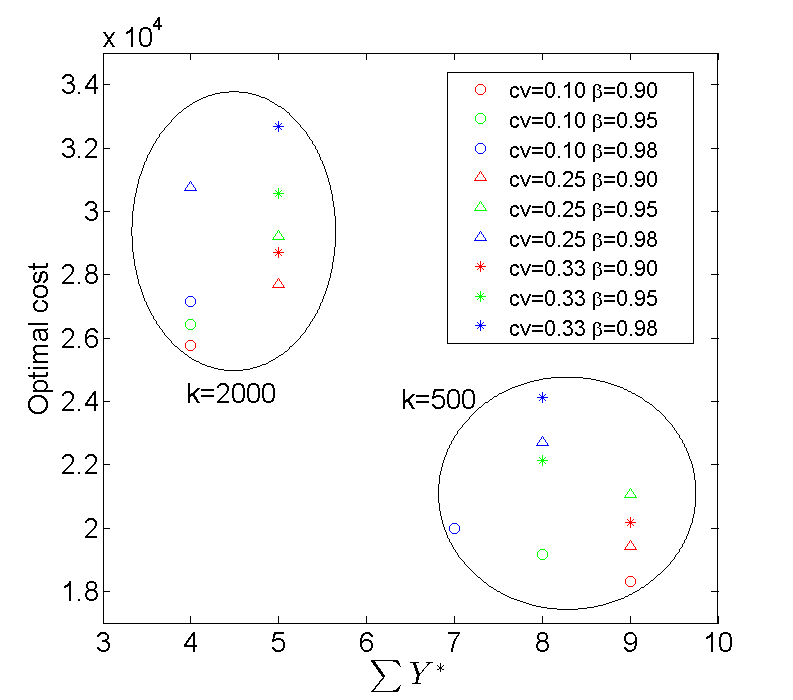
\includegraphics[scale=0.3]{iccsa2015/figures/experimentos.png}
%\includegraphics[scale=0.3]{qnbeta.pdf}
\caption{Optimal cost and its number of ordering periods for $Y^*$ for every instance. Circles represent $cv=0.10$, triangles represent $cv=0.25$ and asterisks $cv=0.33$. The values of $\beta$ are $0.90$, $0.95$ and $0.98$ for each case, (colors: red, green and blue, respectively). $k$ identifies the ordering cost. For simplicity, optimal costs have been group by the value of $k$.}
\label{fig:tests}
\end{figure}




%Looking at the tables it can also be noticed the independence of the optimal quantities with the objective function parameter $k$: for instance, cases like $\beta=0.90$ and $cv=0.25$, $\beta=0.95$ and $cv=0.25$, $\beta=0.95$ and $cv=0.33$, we have that for $k=1000$ and $k=2000$ the best timing vector is the same and hence, the optimal quantities, although total cost obviously change.

Our Algorithm \ref{alg:bestY} has been compared to \emph{fmincon} in terms of performance. In order to obtain runtimes independently on the parameters, Algorithm \ref{alg:bestY} has been run without considering the existence of a lower bound function (line \ref{bestY:line:LB}), optimizing all feasible policies. For the Example \ref{ex:mainexample}, our solver
outperforms the \emph{fmincon} solver in a factor of $20\times$. The main reason for that is that our algorithm is customized for this problem. It makes our algorithm more suitable for solving this kind of problems.

%It is mainly due to the fact that less simulations are needed when using our Proposition~\ref{prop:optimizeY}: to obtain the quantity of a cycle we only need to simulate the evolution of inventory for these periods and once its value is calculated we do not need to update it anymore.
%\subsection{Effectiveness}

%Elapsed time is 2681.157377 seconds./ Elapsed time is  134.266289 seconds.
%Para 13 periodos (un ultimo de mu=500): Elapsed time is 4993.950759 seconds./ Elapsed time is 297.714495 seconds.

\section{Conclusions}
\label{sec:conclusions}
A MINLP model has been presented to determine order quantities for a perishable product inventory control problem. Basic order quantities can be determined to provide feasible production quantities for different delivery policies of the model. Subject to a feasible order timing vector $Y$, a method for finding optimal quantities for the objective function (\ref{eq:obj}) has been devised. For real applications, when $T$ is not very large, this method is able to find the optimal solution for the problem by exhaustive search of feasible policies, using a lower bound function on cost to reduce enumeration.
Moreover, obtained results have shown that our method can reduce the runtime in a factor of $20\times$ with respect to the general Matlab function \emph{fmincon} for solving NLP problems.


Taking into account that the NLP optimizations solved by Algorithm~\ref{alg:optimalforY} are independent, our future works will address the parallelization of the model. This parallelization will allow to obtain more accurate results due to the possibility of  increasing the number of Monte Carlo simulations to solve a particular problem and simultaneously reducing the runtime.



%--------------------------------------------------------------------------

%\subsubsection*{Acknowledgments.}
%This paper has been supported by The Spanish Ministry  (TIN2012-37483) and Junta de Andaluc\'{\i}a (P11-TIC-7176), in part financed by the European Regional Development Fund (ERDF). The study is co-funded by the TIFN (project RE002).

%\bibliographystyle{plain}
%\bibliography{bibtex}

%\end{document}



This translates into a high computational demand. Focusing on speed up the optimization, for instance by using parallel implementations of the algorithm, can be a line of future work.

%\green{ESTO TIENE QUE MIRARSE BIEN The next question is to determine a lower bound for the sum of the order quantities $Q_t$, $t=1,\ldots,T$. Due to the $\beta$ service level constraint, the total quantity needed are lower when more orders are placed. For that reason, we consider the minimum production quantity needed (given by Proposition \ref{prop:optimizeY}) for the timing vector $Y=(1,\ldots,1)$, when an order is placed at every period, as a lower bound for the sum of the quantities of vector $Q$.}

\newpage

\begin{table}[bth!]
\begin{tabular}{cccccc}
\multicolumn{6}{c}{$k=500$ and $\beta=0.9$}                                                                                                                                                                                                                                                                                                                                                \\ \hline
\multicolumn{2}{c}{$cv=0.1$}                                                                                             & \multicolumn{2}{c}{$cv=0.25$}                                                                                             & \multicolumn{2}{c}{$cv=0,33$}                                                                                           \\ \hline
\multicolumn{1}{l}{fmincon}                                & \multicolumn{1}{l|}{Algorithm \ref{alg:optimalforY}}                                 & \multicolumn{1}{l}{fmincon}                                 & \multicolumn{1}{l|}{Algorithm \ref{alg:optimalforY}}                                 & \multicolumn{1}{l}{fmincon}                                & \multicolumn{1}{l}{Algorithm \ref{alg:optimalforY}}                                 \\
728,1548738                                                & \multicolumn{1}{c|}{728,1543455}                            & 804,7278534                                                 & \multicolumn{1}{c|}{804,7281868}                            & 852,5832681                                                & 852,5838539                                                \\
1190,655938                                                & \multicolumn{1}{c|}{1190,655995}                            & 888,623072                                                  & \multicolumn{1}{c|}{888,6229523}                            & 919,2940122                                                & 919,2926353                                                \\
0                                                          & \multicolumn{1}{c|}{0}                                      & 1028,220676                                                 & \multicolumn{1}{c|}{1028,220672}                            & 1059,325366                                                & 1059,325791                                                \\
763,2764977                                                & \multicolumn{1}{c|}{763,2773418}                            & 0                                                           & \multicolumn{1}{c|}{0}                                      & 0                                                          & 0                                                          \\
981,9987407                                                & \multicolumn{1}{c|}{981,9986435}                            & 722,9083453                                                 & \multicolumn{1}{c|}{722,9083722}                            & 712,4241279                                                & 712,4246247                                                \\
0                                                          & \multicolumn{1}{c|}{0}                                      & 735,5299979                                                 & \multicolumn{1}{c|}{735,5300385}                            & 730,6118726                                                & 730,6122459                                                \\
539,018276                                                 & \multicolumn{1}{c|}{539,0182258}                            & 0                                                           & \multicolumn{1}{c|}{0}                                      & 0                                                          & 0                                                          \\
710,9900037                                                & \multicolumn{1}{c|}{710,9899779}                            & 715,1224388                                                 & \multicolumn{1}{c|}{715,1225767}                            & 724,8083083                                                & 724,8082355                                                \\
809,9756847                                                & \multicolumn{1}{c|}{809,9756693}                            & 821,1798169                                                 & \multicolumn{1}{c|}{821,1797793}                            & 835,3303726                                                & 835,3310235                                                \\
442,0447969                                                & \multicolumn{1}{c|}{442,0450676}                            & 460,4714838                                                 & \multicolumn{1}{c|}{460,4715969}                            & 471,8039626                                                & 471,8037974                                                \\
0                                                          & \multicolumn{1}{c|}{0}                                      & 0                                                           & \multicolumn{1}{c|}{0}                                      & 0                                                          & 0                                                          \\
528,78392                                                  & \multicolumn{1}{c|}{528,7838041}                            & 509,0934655                                                 & \multicolumn{1}{c|}{509,0933859}                            & 507,9641154                                                & 507,9639715                                                \\ \hline
\begin{tabular}[c]{@{}c@{}}Cost\\ 18318,47626\end{tabular} & \begin{tabular}[c]{@{}c@{}}Cost \\ 18318,47732\end{tabular} & \begin{tabular}[c]{@{}c@{}}Cost \\ 19422,91505\end{tabular} & \begin{tabular}[c]{@{}c@{}}Cost \\ 19422,91635\end{tabular} & \begin{tabular}[c]{@{}c@{}}Cost\\ 20185,69167\end{tabular} & \begin{tabular}[c]{@{}c@{}}Cost\\ 20185,69422\end{tabular}
\end{tabular}
\end{table}

\begin{table}[bth!]
\begin{tabular}{cccccc}
\multicolumn{6}{c}{$k=500$ and $\beta=0.95$}                                                                                                                                                                                                                                                                                                                                 \\ \hline
\multicolumn{2}{c}{$cv=0.10$}                                                                                           & \multicolumn{2}{c}{$cv=0.25$}                                                                                            & \multicolumn{2}{c}{$cv=0.33$}                                                                                           \\ \hline
\multicolumn{1}{l}{fmincon}                                & \multicolumn{1}{l|}{Algorithm \ref{alg:optimalforY}
}                                & \multicolumn{1}{l}{fmincon}                                 & \multicolumn{1}{l|}{Algorithm \ref{alg:optimalforY}
}                                & \multicolumn{1}{l}{fmincon}                                & \multicolumn{1}{l}{Algorithm \ref{alg:optimalforY}
}                                 \\
784,601074                                                 & \multicolumn{1}{c|}{784,6010978}                           & 905,66832                                                   & \multicolumn{1}{c|}{905,6682038}                           & 974,9879859                                                & 974,987761                                                 \\
1222,634967                                                & \multicolumn{1}{c|}{1222,634083}                           & 1371,176828                                                 & \multicolumn{1}{c|}{1371,176847}                           & 1465,992928                                                & 1465,992825                                                \\
0                                                          & \multicolumn{1}{c|}{0}                                     & 0                                                           & \multicolumn{1}{c|}{0}                                     & 0                                                          & 0                                                          \\
805,7834913                                                & \multicolumn{1}{c|}{805,7844745}                           & 776,69361                                                   & \multicolumn{1}{c|}{776,6936628}                           & 776,754218                                                 & 776,7555805                                                \\
1001,492089                                                & \multicolumn{1}{c|}{1001,491832}                           & 753,2051163                                                 & \multicolumn{1}{c|}{753,2051216}                           & 750,3036009                                                & 750,3031398                                                \\
0                                                          & \multicolumn{1}{c|}{0}                                     & 768,2060009                                                 & \multicolumn{1}{c|}{768,2060042}                           & 766,0852335                                                & 766,0852578                                                \\
1371,234144                                                & \multicolumn{1}{c|}{1371,234274}                           & 0                                                           & \multicolumn{1}{c|}{0}                                     & 0                                                          & 0                                                          \\
0                                                          & \multicolumn{1}{c|}{0}                                     & 761,57545                                                   & \multicolumn{1}{c|}{761,5726035}                           & 778,8816097                                                & 778,8804706                                                \\
841,6764557                                                & \multicolumn{1}{c|}{841,6762581}                           & 871,6922869                                                 & \multicolumn{1}{c|}{871,6926935}                           & 899,4613518                                                & 899,4617583                                                \\
450,5849984                                                & \multicolumn{1}{c|}{450,5850209}                           & 473,3629759                                                 & \multicolumn{1}{c|}{473,3636739}                           & 1052,100997                                                & 1052,101093                                                \\
0                                                          & \multicolumn{1}{c|}{0}                                     & 0                                                           & \multicolumn{1}{c|}{0}                                     & 0                                                          & 0                                                          \\
551,3625707                                                & \multicolumn{1}{c|}{551,3626066}                           & 538,0986876                                                 & \multicolumn{1}{c|}{538,0989586}                           & 0                                                          & 0                                                          \\ \hline
\begin{tabular}[c]{@{}c@{}}Cost\\ 19149,77412\end{tabular} & \begin{tabular}[c]{@{}c@{}}Cost\\ 19149,77275\end{tabular} & \begin{tabular}[c]{@{}c@{}}Cost \\ 21072,39335\end{tabular} & \begin{tabular}[c]{@{}c@{}}Cost\\ 21072,38794\end{tabular} & \begin{tabular}[c]{@{}c@{}}Cost\\ 22141,64843\end{tabular} & \begin{tabular}[c]{@{}c@{}}Cost\\ 22141,64853\end{tabular}
\end{tabular}
\end{table}

\begin{table}[h]
\begin{tabular}{cccccc}
\multicolumn{6}{c}{$k=500$ and $\beta=0.98$}                                                                                                                                                                                                                                                                                                                                  \\ \hline
\multicolumn{2}{c}{$cv=0.1$}                                                                                            & \multicolumn{2}{c}{$cv=0.25$}                                                                                            & \multicolumn{2}{c}{$cv=0.33$}                                                                                            \\ \hline
fmincon                                                    & \multicolumn{1}{c|}{Algorithm \ref{alg:optimalforY}
}                                & \multicolumn{1}{c|}{fmincon}                                & \multicolumn{1}{c|}{Algorithm \ref{alg:optimalforY}
}                                & fmincon                                                     & Algorithm \ref{alg:optimalforY}
                                                     \\
839,1665372                                                & \multicolumn{1}{c|}{839,1665315}                           & 1017,004227                                                 & \multicolumn{1}{c|}{1017,00083}                            & 1106,882177                                                 & 1106,879097                                                \\
1251,378505                                                & \multicolumn{1}{c|}{1251,376864}                           & 1422,665458                                                 & \multicolumn{1}{c|}{1422,667588}                           & 1543,919107                                                 & 1543,919426                                                \\
0                                                          & \multicolumn{1}{c|}{0}                                     & 0                                                           & \multicolumn{1}{c|}{0}                                     & 0                                                           & 0                                                          \\
842,8736583                                                & \multicolumn{1}{c|}{842,8713059}                           & 834,232172                                                  & \multicolumn{1}{c|}{834,233122}                            & 852,2038578                                                 & 852,2054701                                                \\
1016,146562                                                & \multicolumn{1}{c|}{1016,14776}                            & 1136,193173                                                 & \multicolumn{1}{c|}{1136,188437}                           & 801,6791845                                                 & 801,6799582                                                \\
0                                                          & \multicolumn{1}{c|}{0}                                     & 0                                                           & \multicolumn{1}{c|}{0}                                     & 797,18086                                                   & 797,1833083                                                \\
1404,478264                                                & \multicolumn{1}{c|}{1404,481811}                           & 537,5246145                                                 & \multicolumn{1}{c|}{537,5298613}                           & 0                                                           & 0                                                          \\
0                                                          & \multicolumn{1}{c|}{0}                                     & 782,0330036                                                 & \multicolumn{1}{c|}{782,0321725}                           & 834,8421669                                                 & 834,8412525                                                \\
1248,257106                                                & \multicolumn{1}{c|}{1248,256137}                           & 915,0009923                                                 & \multicolumn{1}{c|}{915,0006152}                           & 951,7875855                                                 & 951,7899656                                                \\
0                                                          & \multicolumn{1}{c|}{0}                                     & 1076,222759                                                 & \multicolumn{1}{c|}{1076,223803}                           & 1092,158718                                                 & 1092,156052                                                \\
700,0327939                                                & \multicolumn{1}{c|}{700,0329052}                           & 0                                                           & \multicolumn{1}{c|}{0}                                     & 0                                                           & 0                                                          \\
0                                                          & \multicolumn{1}{c|}{0}                                     & 0                                                           & \multicolumn{1}{c|}{0}                                     & 0                                                           & 0                                                          \\ \hline
\begin{tabular}[c]{@{}c@{}}Cost\\ 19996,68587\end{tabular} & \begin{tabular}[c]{@{}c@{}}Cost\\ 19996,68264\end{tabular} & \begin{tabular}[c]{@{}c@{}}Cost \\ 22712,26446\end{tabular} & \begin{tabular}[c]{@{}c@{}}Cost \\ 22712,2634\end{tabular} & \begin{tabular}[c]{@{}c@{}}Cost \\ 24119,76352\end{tabular} & \begin{tabular}[c]{@{}c@{}}Cost\\ 24119,76651\end{tabular}
\end{tabular}
\end{table}



\begin{table}[h]
\begin{tabular}{cccccc}
\multicolumn{6}{c}{$k=1000$ and $\beta=0.90$}                                                                                                                                                                                                                                                                                \\ \hline
\multicolumn{2}{c}{$cv=0.10$}                                                                                           & \multicolumn{2}{c}{$cv=0.25$}                                                                                           & \multicolumn{2}{c}{$cv=0.33$}                                            \\ \hline
fmincon                                                    & \multicolumn{1}{c|}{Algorithm \ref{alg:optimalforY}
}                                & fmincon                                                    & \multicolumn{1}{c|}{Algorithm \ref{alg:optimalforY}
}                                & fmincon                                                    & Algorithm \ref{alg:optimalforY}
      \\
1676,245566                                                & \multicolumn{1}{c|}{1676,245542}                           & 1816,570638                                                & \multicolumn{1}{c|}{1816,571283}                           & 1909,286292                                                & 1909,286289 \\
0                                                          & \multicolumn{1}{c|}{0}                                     & 0                                                          & \multicolumn{1}{c|}{0}                                     & 0                                                          & 0           \\
1005,207077                                                & \multicolumn{1}{c|}{1005,207083}                           & 1027,349434                                                & \multicolumn{1}{c|}{1027,349396}                           & 1082,085006                                                & 1082,084645 \\
0                                                          & \multicolumn{1}{c|}{0}                                     & 0                                                          & \multicolumn{1}{c|}{0}                                     & 0                                                          & 0           \\
1547,111163                                                & \multicolumn{1}{c|}{1547,11116}                            & 1626,050898                                                & \multicolumn{1}{c|}{1626,051187}                           & 1648,600153                                                & 1648,600208 \\
0                                                          & \multicolumn{1}{c|}{0}                                     & 0                                                          & \multicolumn{1}{c|}{0}                                     & 0                                                          & 0           \\
0                                                          & \multicolumn{1}{c|}{0}                                     & 0                                                          & \multicolumn{1}{c|}{0}                                     & 0                                                          & 0           \\
1632,510758                                                & \multicolumn{1}{c|}{1632,510743}                           & 1762,756308                                                & \multicolumn{1}{c|}{1762,75733}                            & 1867,06339                                                 & 1867,063321 \\
0                                                          & \multicolumn{1}{c|}{0}                                     & 0                                                          & \multicolumn{1}{c|}{0}                                     & 0                                                          & 0           \\
983,4111772                                                & \multicolumn{1}{c|}{983,4111804}                           & 987,6208405                                                & \multicolumn{1}{c|}{987,6209951}                           & 1010,621026                                                & 1010,621371 \\
0                                                          & \multicolumn{1}{c|}{0}                                     & 0                                                          & \multicolumn{1}{c|}{0}                                     & 0                                                          & 0           \\
0                                                          & \multicolumn{1}{c|}{0}                                     & 0                                                          & \multicolumn{1}{c|}{0}                                     & 0                                                          & 0           \\ \hline
\begin{tabular}[c]{@{}c@{}}Cost\\ 21303,09318\end{tabular} & \begin{tabular}[c]{@{}c@{}}Cost\\ 21303,09306\end{tabular} & \begin{tabular}[c]{@{}c@{}}Cost\\ 22684,52416\end{tabular} & \begin{tabular}[c]{@{}c@{}}Cost\\ 22684,53058\end{tabular} & \begin{tabular}[c]{@{}c@{}}Cost\\ 23703,59471\end{tabular} & 23703,59445
\end{tabular}
\end{table}

\begin{table}[h]
\begin{tabular}{cccccc}
\multicolumn{6}{c}{$k=1000$ and $\beta=0.95$}                                                                                                                                                                                                                                                                                                                                \\ \hline
\multicolumn{2}{c}{$cv=0.10$}                                                                                           & \multicolumn{2}{c}{$cv=0.25$}                                                                                           & \multicolumn{2}{c|}{$cv=0.33$}                                                                                           \\ \hline
fmincon                                                    & \multicolumn{1}{c|}{Algorithm \ref{alg:optimalforY}
}                                & fmincon                                                    & \multicolumn{1}{c|}{Algorithm \ref{alg:optimalforY}
}                                & fmincon                                                    & Algorithm \ref{alg:optimalforY}
                                                      \\
1755,123897                                                & \multicolumn{1}{c|}{1755,123777}                           & 1957,495653                                                & \multicolumn{1}{c|}{1957,495951}                           & 2087,09391                                                 & 2087,09401                                                  \\
0                                                          & \multicolumn{1}{c|}{0}                                     & 0                                                          & \multicolumn{1}{c|}{0}                                     & 0                                                          & 0                                                           \\
1051,676644                                                & \multicolumn{1}{c|}{1051,676656}                           & 1111,46131                                                 & \multicolumn{1}{c|}{1111,461284}                           & 1193,598758                                                & 1193,598731                                                 \\
0                                                          & \multicolumn{1}{c|}{0}                                     & 0                                                          & \multicolumn{1}{c|}{0}                                     & 0                                                          & 0                                                           \\
1590,053265                                                & \multicolumn{1}{c|}{1590,054118}                           & 1695,109158                                                & \multicolumn{1}{c|}{1695,109129}                           & 1725,290363                                                & 1725,29249                                                  \\
0                                                          & \multicolumn{1}{c|}{0}                                     & 0                                                          & \multicolumn{1}{c|}{0}                                     & 0                                                          & 0                                                           \\
0                                                          & \multicolumn{1}{c|}{0}                                     & 0                                                          & \multicolumn{1}{c|}{0}                                     & 0                                                          & 0                                                           \\
1708,032315                                                & \multicolumn{1}{c|}{1708,031831}                           & 1900,283406                                                & \multicolumn{1}{c|}{1900,283613}                           & 2037,08966                                                 & 2037,08967                                                  \\
0                                                          & \multicolumn{1}{c|}{0}                                     & 0                                                          & \multicolumn{1}{c|}{0}                                     & 0                                                          & 0                                                           \\
1014,817609                                                & \multicolumn{1}{c|}{1014,81775}                            & 1034,719166                                                & \multicolumn{1}{c|}{1034,718994}                           & 1066,283782                                                & 1066,28411                                                  \\
0                                                          & \multicolumn{1}{c|}{0}                                     & 0                                                          & \multicolumn{1}{c|}{0}                                     & 0                                                          & 0                                                           \\
0                                                          & \multicolumn{1}{c|}{0}                                     & 0                                                          & \multicolumn{1}{c|}{0}                                     & 0                                                          & 0                                                           \\ \hline
\begin{tabular}[c]{@{}c@{}}Cost\\ 22149,21714\end{tabular} & \begin{tabular}[c]{@{}c@{}}Cost\\ 22149,21816\end{tabular} & \begin{tabular}[c]{@{}c@{}}Cost\\ 24210,28601\end{tabular} & \begin{tabular}[c]{@{}c@{}}Cost\\ 24210,28695\end{tabular} & \begin{tabular}[c]{@{}c@{}}Cost\\ 25578,13739\end{tabular} & \begin{tabular}[c]{@{}c@{}}Cost \\ 25578,14501\end{tabular}
\end{tabular}
\end{table}

\begin{table}[h]
\begin{tabular}{cccccc}
\hline
\multicolumn{6}{c}{$k=1000$ and $\beta=0.98$}                                                                                                                                                                                                                                                                                                                                 \\ \hline
\multicolumn{2}{c}{$cv=0.10$}                                                                                             & \multicolumn{2}{c}{$cv=0.25$}                                                                                          & \multicolumn{2}{c}{$0.33$}                                                                                               \\ \hline
fmincon                                                     & \multicolumn{1}{c|}{Algorithm \ref{alg:optimalforY}
}                                 & fmincon                                                    & \multicolumn{1}{c|}{Algorithm \ref{alg:optimalforY}
}                               & fmincon                                                    & Algorithm \ref{alg:optimalforY}
                                                      \\
1832,973797                                                 & \multicolumn{1}{c|}{1832,973599}                            & 2108,055296                                                & \multicolumn{1}{c|}{2108,049892}                          & 2281,203157                                                & 2281,20253                                                  \\
0                                                           & \multicolumn{1}{c|}{0}                                      & 0                                                          & \multicolumn{1}{c|}{0}                                    & 0                                                          & 0                                                           \\
1091,838476                                                 & \multicolumn{1}{c|}{1091,838483}                            & 1200,624005                                                & \multicolumn{1}{c|}{1200,625875}                          & 1321,217184                                                & 1321,217301                                                 \\
0                                                           & \multicolumn{1}{c|}{0}                                      & 0                                                          & \multicolumn{1}{c|}{0}                                    & 0                                                          & 0                                                           \\
1623,811545                                                 & \multicolumn{1}{c|}{1623,811266}                            & 1769,145677                                                & \multicolumn{1}{c|}{1769,145317}                          & 1221,382227                                                & 1221,382239                                                 \\
0                                                           & \multicolumn{1}{c|}{0}                                      & 0                                                          & \multicolumn{1}{c|}{0}                                    & 0                                                          & 0                                                           \\
0                                                           & \multicolumn{1}{c|}{0}                                      & 0                                                          & \multicolumn{1}{c|}{0}                                    & 1464,506958                                                & 1464,512029                                                 \\
1784,527781                                                 & \multicolumn{1}{c|}{1784,526698}                            & 2048,277839                                                & \multicolumn{1}{c|}{2048,2763}                            & 0                                                          & 0                                                           \\
0                                                           & \multicolumn{1}{c|}{0}                                      & 0                                                          & \multicolumn{1}{c|}{0}                                    & 950,0369915                                                & 950,0398833                                                 \\
1039,321033                                                 & \multicolumn{1}{c|}{1039,321302}                            & 1080,706839                                                & \multicolumn{1}{c|}{1080,711031}                          & 1092,826693                                                & 1092,821389                                                 \\
0                                                           & \multicolumn{1}{c|}{0}                                      & 0                                                          & \multicolumn{1}{c|}{0}                                    & 0                                                          & 0                                                           \\
0                                                           & \multicolumn{1}{c|}{0}                                      & 0                                                          & \multicolumn{1}{c|}{0}                                    & 0                                                          & 0                                                           \\ \hline
\begin{tabular}[c]{@{}c@{}}Cost \\ 23008,57012\end{tabular} & \begin{tabular}[c]{@{}c@{}}Cost \\ 23008,56545\end{tabular} & \begin{tabular}[c]{@{}c@{}}Cost\\ 25866,26122\end{tabular} & \begin{tabular}[c]{@{}c@{}}Cost\\ 25866,2571\end{tabular} & \begin{tabular}[c]{@{}c@{}}Cost\\ 27601,91143\end{tabular} & \begin{tabular}[c]{@{}c@{}}Cost \\ 27601,92196\end{tabular} \\ \hline
\end{tabular}
\end{table}



\begin{table}[h]
\begin{tabular}{cccccc}
\multicolumn{6}{c}{$k=2000$ and $\beta=0.90$}                                                                                                                                                                                                                                                                                                                                     \\ \hline
\multicolumn{2}{c}{$cv=0.10$}                                                                                             & \multicolumn{2}{c}{$cv=0.25$}                                                                                             & \multicolumn{2}{c}{$cv=0.33$}                                                                                             \\ \hline
fmincon                                                     & \multicolumn{1}{c|}{Algorithm \ref{alg:optimalforY}
}                                 & fmincon                                                     & \multicolumn{1}{c|}{Algorithm \ref{alg:optimalforY}
}                                 & fmincon                                                     & Algorithm \ref{alg:optimalforY}
                                                      \\
2028,679335                                                 & \multicolumn{1}{c|}{2028,679313}                            & 1816,570638                                                 & \multicolumn{1}{c|}{1816,571283}                            & 1909,286292                                                 & 1909,286289                                                 \\
0                                                           & \multicolumn{1}{c|}{0}                                      & 0                                                           & \multicolumn{1}{c|}{0}                                      & 0                                                           & 0                                                           \\
0                                                           & \multicolumn{1}{c|}{0}                                      & 1027,349434                                                 & \multicolumn{1}{c|}{1027,349396}                            & 1082,085006                                                 & 1082,084645                                                 \\
1938,161733                                                 & \multicolumn{1}{c|}{1938,161663}                            & 0                                                           & \multicolumn{1}{c|}{0}                                      & 0                                                           & 0                                                           \\
0                                                           & \multicolumn{1}{c|}{0}                                      & 1626,050898                                                 & \multicolumn{1}{c|}{1626,051187}                            & 1648,600153                                                 & 1648,600208                                                 \\
0                                                           & \multicolumn{1}{c|}{0}                                      & 0                                                           & \multicolumn{1}{c|}{0}                                      & 0                                                           & 0                                                           \\
2291,71704                                                  & \multicolumn{1}{c|}{2291,717331}                            & 0                                                           & \multicolumn{1}{c|}{0}                                      & 0                                                           & 0                                                           \\
0                                                           & \multicolumn{1}{c|}{0}                                      & 1762,756308                                                 & \multicolumn{1}{c|}{1762,75733}                             & 1867,06339                                                  & 1867,063321                                                 \\
0                                                           & \multicolumn{1}{c|}{0}                                      & 0                                                           & \multicolumn{1}{c|}{0}                                      & 0                                                           & 0                                                           \\
997,750003                                                  & \multicolumn{1}{c|}{997,7499503}                            & 987,6208405                                                 & \multicolumn{1}{c|}{987,6209951}                            & 1010,621026                                                 & 1010,621371                                                 \\
0                                                           & \multicolumn{1}{c|}{0}                                      & 0                                                           & \multicolumn{1}{c|}{0}                                      & 0                                                           & 0                                                           \\
0                                                           & \multicolumn{1}{c|}{0}                                      & 0                                                           & \multicolumn{1}{c|}{0}                                      & 0                                                           & 0                                                           \\ \hline
\begin{tabular}[c]{@{}c@{}}Cost \\ 25769,18772\end{tabular} & \begin{tabular}[c]{@{}c@{}}Cost \\ 25769,18815\end{tabular} & \begin{tabular}[c]{@{}c@{}}Cost \\ 27684,52416\end{tabular} & \begin{tabular}[c]{@{}c@{}}Cost \\ 27684,53058\end{tabular} & \begin{tabular}[c]{@{}c@{}}Cost \\ 28703,59471\end{tabular} & \begin{tabular}[c]{@{}c@{}}Cost \\ 28703,59445\end{tabular}
\end{tabular}
\end{table}

\begin{table}[h]
\begin{tabular}{cccccc}
\multicolumn{6}{c}{$k=2000$ and $\beta=0.95$}                                                                                                                                                                                                                                                                                                                                   \\ \hline
\multicolumn{2}{c}{$cv=0.10$}                                                                                             & \multicolumn{2}{c}{$cv=0.25$}                                                                                             & \multicolumn{2}{c}{$cv=0.33$}                                                                                             \\ \hline
fmincon                                                     & \multicolumn{1}{c|}{Algorithm \ref{alg:optimalforY}
}                                 & fmincon                                                     & \multicolumn{1}{c|}{Algorithm \ref{alg:optimalforY}
}                                 & fmincon                                                     & Algorithm \ref{alg:optimalforY}
                                                      \\
2078,265295                                                 & \multicolumn{1}{c|}{2078,265295}                            & 1957,495653                                                 & \multicolumn{1}{c|}{1957,495951}                            & 2087,09391                                                  & 2087,09401                                                  \\
0                                                           & \multicolumn{1}{c|}{0}                                      & 0                                                           & \multicolumn{1}{c|}{0}                                      & 0                                                           & 0                                                           \\
0                                                           & \multicolumn{1}{c|}{0}                                      & 1111,46131                                                  & \multicolumn{1}{c|}{1111,461284}                            & 1193,598758                                                 & 1193,598731                                                 \\
1984,12144                                                  & \multicolumn{1}{c|}{1984,121441}                            & 0                                                           & \multicolumn{1}{c|}{0}                                      & 0                                                           & 0                                                           \\
0                                                           & \multicolumn{1}{c|}{0}                                      & 1695,109158                                                 & \multicolumn{1}{c|}{1695,109129}                            & 1725,290362                                                 & 1725,29249                                                  \\
0                                                           & \multicolumn{1}{c|}{0}                                      & 0                                                           & \multicolumn{1}{c|}{0}                                      & 0                                                           & 0                                                           \\
2373,28118                                                  & \multicolumn{1}{c|}{2373,28118}                             & 0                                                           & \multicolumn{1}{c|}{0}                                      & 0                                                           & 0                                                           \\
0                                                           & \multicolumn{1}{c|}{0}                                      & 1900,283406                                                 & \multicolumn{1}{c|}{1900,283613}                            & 2037,08966                                                  & 2037,08967                                                  \\
0                                                           & \multicolumn{1}{c|}{0}                                      & 0                                                           & \multicolumn{1}{c|}{0}                                      & 0                                                           & 0                                                           \\
1043,495293                                                 & \multicolumn{1}{c|}{1043,495293}                            & 1034,719166                                                 & \multicolumn{1}{c|}{1034,718994}                            & 1066,283782                                                 & 1066,28411                                                  \\
0                                                           & \multicolumn{1}{c|}{0}                                      & 0                                                           & \multicolumn{1}{c|}{0}                                      & 0                                                           & 0                                                           \\
0                                                           & \multicolumn{1}{c|}{0}                                      & 0                                                           & \multicolumn{1}{c|}{0}                                      & 0                                                           & 0                                                           \\ \hline
\begin{tabular}[c]{@{}c@{}}Cost \\ 26437,16379\end{tabular} & \begin{tabular}[c]{@{}c@{}}Cost \\ 26437,16379\end{tabular} & \begin{tabular}[c]{@{}c@{}}Cost \\ 29210,28601\end{tabular} & \begin{tabular}[c]{@{}c@{}}Cost \\ 29210,28695\end{tabular} & \begin{tabular}[c]{@{}c@{}}Cost \\ 30578,13739\end{tabular} & \begin{tabular}[c]{@{}c@{}}Cost \\ 30578,14501\end{tabular}
\end{tabular}
\end{table}

\begin{table}[h]
\begin{tabular}{cccccc}
\multicolumn{6}{c}{$k=2000$ and $\beta=0.98$}                                                                                                                                                                                                                                                                                    \\ \hline
\multicolumn{2}{c}{$cv=0.10$}                                                                                            & \multicolumn{2}{c}{$cv=0.25$}                                                                                             & \multicolumn{2}{c}{$cv=0.33$}                                             \\ \hline
fmincon                                                     & \multicolumn{1}{c|}{Algorithm \ref{alg:optimalforY}
}                                & fmincon                                                     & \multicolumn{1}{c|}{Algorithm \ref{alg:optimalforY}
}                                 & fmincon                                                     & Algorithm \ref{alg:optimalforY}
      \\
2133,605803                                                 & \multicolumn{1}{c|}{2133,605059}                           & 2499,387255                                                 & \multicolumn{1}{c|}{2499,387255}                            & 2281,203157                                                 & 2281,20253  \\
0                                                           & \multicolumn{1}{c|}{0}                                     & 0                                                           & \multicolumn{1}{c|}{0}                                      & 0                                                           & 0           \\
0                                                           & \multicolumn{1}{c|}{0}                                     & 0                                                           & \multicolumn{1}{c|}{0}                                      & 1321,217184                                                 & 1321,217301 \\
2038,650586                                                 & \multicolumn{1}{c|}{2038,648815}                           & 2412,338355                                                 & \multicolumn{1}{c|}{2412,338356}                            & 0                                                           & 0           \\
0                                                           & \multicolumn{1}{c|}{0}                                     & 0                                                           & \multicolumn{1}{c|}{0}                                      & 1809,347095                                                 & 1809,344111 \\
0                                                           & \multicolumn{1}{c|}{0}                                     & 0                                                           & \multicolumn{1}{c|}{0}                                      & 0                                                           & 0           \\
2456,00282                                                  & \multicolumn{1}{c|}{2455,999666}                           & 2768,80475                                                  & \multicolumn{1}{c|}{2768,80475}                             & 0                                                           & 0           \\
0                                                           & \multicolumn{1}{c|}{0}                                     & 0                                                           & \multicolumn{1}{c|}{0}                                      & 2228,007918                                                 & 2228,00492  \\
0                                                           & \multicolumn{1}{c|}{0}                                     & 0                                                           & \multicolumn{1}{c|}{0}                                      & 0                                                           & 0           \\
1088,694017                                                 & \multicolumn{1}{c|}{1088,69398}                            & 1234,89289                                                  & \multicolumn{1}{c|}{1234,89289}                             & 1120,436169                                                 & 1120,431677 \\
0                                                           & \multicolumn{1}{c|}{0}                                     & 0                                                           & \multicolumn{1}{c|}{0}                                      & 0                                                           & 0           \\
0                                                           & \multicolumn{1}{c|}{0}                                     & 0                                                           & \multicolumn{1}{c|}{0}                                      & 0                                                           & 0           \\ \hline
\begin{tabular}[c]{@{}c@{}}Cost \\ 27150,29893\end{tabular} & \begin{tabular}[c]{@{}c@{}}Cost \\ 27150,2818\end{tabular} & \begin{tabular}[c]{@{}c@{}}Cost \\ 30746,76829\end{tabular} & \begin{tabular}[c]{@{}c@{}}Cost \\ 30746,76829\end{tabular} & \begin{tabular}[c]{@{}c@{}}Cost \\ 32668,46264\end{tabular} & \begin{tabular}[c]{@{}c@{}}Cost \\ 32668,42921\end{tabular}
\end{tabular}
\end{table}
%--------------------------------------------------------------------------
%\section*{Appendix A: Description of the problems}
%\label{Sec:Ap}
